\documentclass[11pt,a4paper,titlepage,oneside]{report}

%%% RELACIÓN DE VARIABLES A PERSONALIZAR %%%
% \def\lingua{gal}
\def\lingua{esp} % descomenta esta liña se redactarás a memoria en español
%\def\lingua{eng} % descomenta esta liña se redactarás a memoria en inglés
\def\nome{David Rodríguez Bacelar}                             % substitúe aquí o teu nome
\def\nomedirectorA{Patricia Martín Rodilla, David Otero Freijeiro}              % substitúe aquí o nome de quen dirixe
%\def\nomedirectorB{Outro Nome Completo}             % duplica esta liña máis veces se o precisas, cambiando
% a letra final (A, B, C, D...): úsanse na portada.tex
\def\titulo{Perfilado automático de usuarios en corpus sociales sobre el movimiento Black Lives Matter} % substitúe aquí o título do teu TFG
%\def\titulacion{gced}                               % descomenta esta liña e comenta a seguinte se es estudante do GCED
\def\titulacion{gei}
\def\mencion{COMPUTACIÓN}
% \def\mencion{ENXEÑARÍA DO SOFTWARE}
%\def\mencion{ENXEÑARÍA DE COMPUTADORES}
%\def\mencion{SISTEMAS DE INFORMACIÓN}
%\def\mencion{TECNOLOXÍAS DA INFORMACIÓN}

\def\renomearcadros{si}

\usepackage{estilo_tfg}

% Lista de paquetes potencialmente interesantes (uso baixo demanda)

\usepackage{fancyvrb}
\fvset{xleftmargin=1em,frame=single,fontsize=\small,numbers=left}
\usepackage{pgfplots}
\pgfplotsset{width=10cm,compat=1.9}
% \usepgfplotslibrary{external}
% \tikzexternalize
% \usepackage{alltt}       % proporciona o entorno alltt, semellante a verbatim pero que respecta comandos
% \usepackage{enumitem}    % permite personalizar os entornos de lista
% \usepackage{eurofont}    % proporciona o comando \euro
\usepackage{float}       % permite máis opcións para controlar obxectos flotantes (táboas, figuras)
% \usepackage{hhline}      % permite personalizar as liñas horizontais en arrays e táboas
\usepackage{longtable}   % permite construir táboas que ocupan máis dunha páxina
% \usepackage{lscape}      % permite colocar partes do documento en orientación apaisada
% \usepackage{moreverb}    % permite personalizar o entorno verbatim
% \usepackage{multirow}    % permite crear celdas que ocupan varias filas da mesma táboa
% \usepackage{pdfpages}    % permite insertar ficheiros en PDF no documento
% \usepackage{rotating}    % permite diferentes tipos de rotacións para figuras e táboas
\usepackage{subcaption}
\usepackage{hhline}
% \usepackage{tabu}        % permite táboas flexibles
% \usepackage{tabularx}    % permite táboas con columnas de anchura determinada
\colorlet{punct}{red!60!black}
\definecolor{background}{HTML}{EEEEEE}
\definecolor{delim}{RGB}{20,105,176}
\colorlet{numb}{magenta!60!black}

\usepackage{sourcecodepro}

\lstdefinelanguage{json}{
    basicstyle=\scriptsize\ttfamily,
    numbers=left,
    numberstyle=\tiny,
    stepnumber=1,
    numbersep=4pt,
    showstringspaces=false,
    breaklines=true,
    frame=none,
    backgroundcolor=\color{background},
    literate=
     *{0}{{{\color{numb}0}}}{1}
      {1}{{{\color{numb}1}}}{1}
      {2}{{{\color{numb}2}}}{1}
      {3}{{{\color{numb}3}}}{1}
      {4}{{{\color{numb}4}}}{1}
      {5}{{{\color{numb}5}}}{1}
      {6}{{{\color{numb}6}}}{1}
      {7}{{{\color{numb}7}}}{1}
      {8}{{{\color{numb}8}}}{1}
      {9}{{{\color{numb}9}}}{1}
      {:}{{{\color{punct}{:}}}}{1}
      {,}{{{\color{punct}{,}}}}{1}
      {\{}{{{\color{delim}{\{}}}}{1}
      {\}}{{{\color{delim}{\}}}}}{1}
      {[}{{{\color{delim}{[}}}}{1}
      {]}{{{\color{delim}{]}}}}{1},
}

%%%%%%%%%%%%%%%%%%%%%%%%%%%%%%%%%%%%%%%%%%%%%%%%%%%%%%%%%%%%%%%%%%%%%%%%%%%%%%%%
% Corpo                                                                        %
%%%%%%%%%%%%%%%%%%%%%%%%%%%%%%%%%%%%%%%%%%%%%%%%%%%%%%%%%%%%%%%%%%%%%%%%%%%%%%%%

\begin{document}

\setlength\arrayrulewidth{0.7pt}

%%%%%%%%%%%%%%%%%%%%%%%%%%%%%%%%%%%%%%%%
% Preliminares do documento            %
%%%%%%%%%%%%%%%%%%%%%%%%%%%%%%%%%%%%%%%%

\include{portada/portada}
\dedicatoria{Dedicatoria} % escribe neste comando o teu texto de dedicatoria
\paxinaenbranco\
\begin{agradecementos}
  \blindtext\                % substitúe este comando polo teu texto de agradecementos
\end{agradecementos}
%%%%%%%%%%%%%%%%%%%%%%%%%%%%%%%%%%%%%%%%%%%%%%%%%%%%%%%%%%%%%%%%%%%%%%%%%%%%%%%%

\pagestyle{empty}
\begin{abstract}
  % Con todo, a lo largo de este trabajo, se profundizará más en el perfilado automático de autores, analizando diferentes algoritmos y su rendimiento,
  % a la vez que se ofrecerá una aplicación web donde se mostrará el resultado del perfilado en un \textit{dashboard} intuitivo y accesible. Además, utilizaremos
  % como caso de uso y análisis la colección de referencia sobre el movimiento \textit{Black Lives Matter (BLM)}, extraída mediante la metodología descrita en \cite{oterorodilla2021}.

  \vspace*{25pt}
  \begin{segundoresumo}
    \blindtext % substitúe este comando polo resumo do teu TFG
               % na lingua secundaria do documento (tipicamente: inglés)
  \end{segundoresumo}
\vspace*{25pt}
\newpage
\begin{multicols}{2}
\begin{description}
\item [\palabraschaveprincipal:] \mbox{} \\[-20pt]
  \begin{itemize}
    \item \textit{Perfilado de autor}
    \item \textit{Redes sociales}
    \item \textit{Procesado de lenguaje natural}
    \item \textit{Aplicación web}
    \item \textit{Aprendizaje automático}
  \end{itemize}
\end{description}

\begin{description}
\item [\palabraschavesecundaria:] \mbox{} \\[-20pt]
  \begin{itemize}
    \item \textit{Author profiling}
    \item \textit{Social networks}
    \item \textit{Natural language processing}
    \item \textit{Web application}
    \item \textit{Machine learning}
  \end{itemize}
\end{description}
\end{multicols}

\end{abstract}
\pagestyle{fancy}

%%%%%%%%%%%%%%%%%%%%%%%%%%%%%%%%%%%%%%%%%%%%%%%%%%%%%%%%%%%%%%%%%%%%%%%%%%%%%%%%


\pagenumbering{roman}
\setcounter{page}{1}
\bstctlcite{IEEEexample:BSTcontrol}

\tableofcontents
\listoffigures
\listoftables
\clearpage

\pagenumbering{arabic}
\setcounter{page}{1}

%%%%%%%%%%%%%%%%%%%%%%%%%%%%%%%%%%%%%%%%
% Capítulos                            %
%%%%%%%%%%%%%%%%%%%%%%%%%%%%%%%%%%%%%%%%

\chapter{Introducción}
\label{chap:introduccion}

\lettrine{A}{partir} de la segunda década de los 2000, las redes sociales han experimentado
un crecimiento continuado de su uso, tanto en número de usuarios como en
cantidad de información generada. Como se muestra en el reporte \textit{"Digital 2023 Global Overview Report"} (We Are Social et al., 2023)
\cite{wearesocial}, a principios del año 2013 existían alrededor de 1.7 millones de usuarios en las redes sociales,
mientras que a principios del año 2023, esta cifra aumentó hasta los 4.7 millones, con una variación anual media del 10.8\% (se puede ver
más información en la Figura \ref{fig:usuarios_redes_sociales}).
Así, plataformas como Facebook, Instagram, Twitter o YouTube, cuentan con millones de usuarios activos diariamente,
donde se comparte información o se crea contenido de entretenimiento. Además, las redes sociales se han convertido en
un lugar donde se debate sobre temas políticos, sociales o económicos, y donde se comparten diversas opiniones y noticias. 
Este hecho se puede ver, de nuevo, en el reporte mecionado anteriormente, donde se muestra que el 34.2\% de los usuarios
de redes sociales las utilizan para informarse sobre noticias, el 28.8\% para saber cuales son los temas de actualidad
y el 23.4\% para compartir opiniones y debatir con otros usuarios.

\bigskip
\begin{figure}[H]
	\centering
	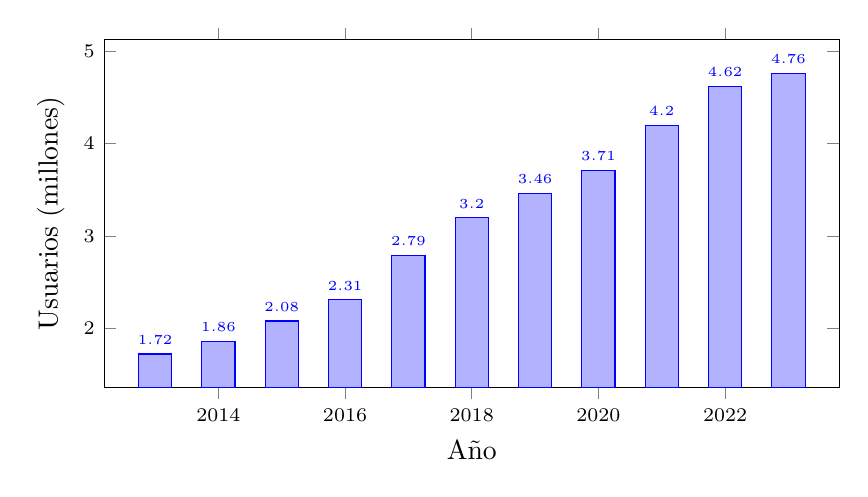
\begin{tikzpicture}
		\begin{axis}[
			width=0.9\textwidth,
			height=6cm,
			xmajorgrids=false,
			x tick label style={/pgf/number format/1000 sep=},
			x tick label style={font=\scriptsize},
			y tick label style={font=\scriptsize},
			ylabel=Usuarios (millones),
			xlabel=Año,
			ybar=6pt,
			bar width=12pt,
			enlarge x limits=0.08,
			enlarge y limits=0.12,
			nodes near coords,
			nodes near coords style={font=\tiny}
		]
		\addplot 
			coordinates {(2013,1.720) (2014,1.857) (2015,2.078)
			(2016,2.307) (2017,2.789) (2018,3.196) (2019,3.461)
			(2020,3.709) (2021,4.199) (2022,4.623) (2023,4.760)};
		\end{axis}
	\end{tikzpicture}
	\caption{Evolución del número de usuarios en redes sociales.}
	\label{fig:usuarios_redes_sociales}
\end{figure}

\section{Importancia de las redes sociales}
\label{sec:intr_importancia}
Toda esta información generada tiene una gran relevancia a distintos niveles. En primer lugar, cabe destacar el impacto que
tienen las redes sociales a nivel político. Y es que en la actualidad, vivimos en una campaña permanente (Blumenthal, 1980)
\cite{sydney1980permanent}, 
donde el acceso a la redes sociales ofrece la posibilidad a los ciudadanos de estar informados sobre política, mientras que a las instituciones
de poder les permite conocer el estado de la opinión pública (Strömbäck, 2008)
\cite{stromback2008four}, pudiendo llegar a influenciar "mucho" o "bastante" la intención de voto (Gallardo-Paúls, 2016) \cite{gallardo2016pseudopolitica}.
En segundo lugar, la información generada en las redes sociales también tiene un gran impacto a nivel social. ¿Quiénes son los
usuarios más activos? ¿Qué género predomina en las redes sociales? ¿Qué edad tienen los usuarios?. Cabe resaltar también el
impacto que tienen las redes sociales a nivel económico, ya que estas plataformas se han convertido en un lugar donde las empresas
publicitan sus productos y servicios y a las que destinan gran parte de sus presupuestos en publicidad 
(Saxena et al., 2013)\cite{saxena2013advertising}. Finalmente, destacar el impacto que tienen las redes sociales a nivel de seguridad,
ya que estas plataformas se han convertido en un lugar donde se comparte información personal, y donde se pueden cometer delitos como
el \textit{cyberbullying} o el \textit{grooming} (Machimbarrena et al., 2018) \cite{machimbarrena2018internet}.

\section{Perfilado de autor}
\label{sec:intro_perfilado}
Surge de esta forma la necesidad de analizar toda la información que se genera y proporiconar así herramientas útiles en todos los niveles vistos en la Sección \ref{sec:intr_importancia}.
En este contexto, el perfilado de autor en redes sociales se ha convertido en un área de investigación de gran interés
en los últimos años, posicionándose como una herramienta de creciente importancia en áreas como la seguridad, el \textit{marketing}
o la investigación forense (Rangel et al., 2013) \cite{rangel2013overview}.

\bigskip
El perfilado de autor, también conocido como \textit{author profiling} en inglés, consiste en determinar, a partir de un texto, 
las características de su autor, como su género, edad, rasgos personales, etc. Para ello se hace uso de diversas técnicas de aprendizaje automático
basadas en NLP (del inglés \textit{Natural Language Processing}), que permiten extraer características lingüísticas del texto y utilizarlas para una
posterior clasificación. Así, el perfilado de autor sería una herramienta de gran ayuda a la hora de realizar
análisis sociales sobre temas específicos; sería muy práctico para empresas que quieran conocer el perfil de los clientes que opinan de 
forma positiva y negativa de sus productos; tendría un gran valor
para los partidos políticos, dado que podrían conocer cuál es el perfil de sus votantes; y sería también de gran utilidad para temas como la evaluación
sospechosos teniendo en cuenta su perfil lingüístico.

\chapter{Estado del arte del perfilado de autor}
\label{chap:estadoarte}

Durante los inicios del perfilado automático de autor, los algoritmos se centraban en la tarea de la clasificación por género.
En esta línea, trabajos como Koppel et al., 2002 \cite{koppel2002automatically} se desmarcaban de la tendencia de la época,
la cual se basaba en la clasificación de textos en base a su contenido, para enfocarse en la clasificación de textos en base a su estilo.
En este caso, se centraban en la obtención del género del autor mediante el análisis
de 920 documentos de carácter formal escritos en inglés con una media de alrededor de 34.300 palabras cada uno, obteniendo una precisión en la clasificación de
aproximadamente el 77\%.

\bigskip
Así, la demostración de la existencia de rasgos diferenciadores en la escritura que permitían perfilar ciertos ascpectos del individuo, especialmente del género, 
supuso un gran avance en el campo del perfilado de autor
y dió pié a la realización de trabajos como (Argamon et al., 2003) \cite{argamon2003gender}, (Corney et.al, 2002) \cite{corney2002gender} o (Otterbacher et al., 2010) \cite{otterbacher2010inferring}, 
así como también permitió el inicio de una clasificación más compleja en base a otras características demográficas.

\bigskip
Posteriormente, en los años siguientes, tal como recoge Wiegmann et al., 2019 \cite{wiegmann2019overview}, se continuarían llevando a cabo estudios en esta línea, diversificando
las características a clasificar. En este sentido, se realizarían trabajos como Álvarez-Carmona et al., 2018 \cite{alvarez2018overview}, donde se buscaba
predecir el lugar de residencia del autor junto a su ocupación; otros como Volkova et al., 2015 \cite{volkova2015predicting}, en el que se trataba de perfilar la orientación política,
el salario, el optimismo del autor o su sentimiento de satisfacción vital; Preoţiuc-Pietro et al., 2018 \cite{preoctiuc2018user}, en el que se llevaba a cabo la tarea de
clasificar la raza y la etnia del autor; u otros como Fatima et al., 2017 \cite{fatima2017multilingual} que buscaban extender el perfilado de autor a otros idiomas. Asimismo,
la mayor parte de los \textit{datasets} utilizados para la creación de los modelos con estos algoritmos, se basaban en textos de redes sociales como Twitter (Burger et al., 2011) \cite{burger2011discriminating},
Facebook (Fatima et al., 2017) \cite{fatima2017multilingual} o Reddit (Gjurković et al., 2018) \cite{gjurkovic2018reddit}, reflejando así la importancia de estas plataformas
en la actualidad.

\bigskip
Por otro lado, en el año 2011, se celebraría el primer evento organizado por el \textit{PAN} (\textit{Plagiarism Analysis, Authorship Identification, and Near-Duplicate Detection}) \cite{pan},
uno de los foro de investigación más importantes que organiza eventos científicos y tareas anuales relacionadas con el análisis forense de textos digitales
y rasgos estilométricos, así como uno de los grandes implusores del perfilado de autor. La primera de las tareas centrada en este campo se celebraría en el año 2013 (Rangel et al., 2013) \cite{rangel2013overview},
en la que se pedía a los participantes que obtuvieran, a partir de una serie de \textit{tweets}, la edad y el género de su autor. El ganador de este concurso obtuvo una
precisión del 60\% en la clasificación de género y del 67\% en la clasificación de edad, haciendo uso, la mayor parte de los participantes, de técnicas de aprendizaje
supervisado como los Árboles de Decisión (en inglés \textit{Decission Trees}) o las Máquinas de Soporte Vectorial (en inglés \textit{Support Vector Machines}) e inluyendo
en sus modelos características basadas en el TF-IDF, n-gramas, etiquetas POS u otras como el número de emoticonos o la frecuencia de signos de puntuación.
En los siguientes años se celebrarían nuevas ediciones con el perfilado de autor en el centro (Rangel et al., 2014 \cite{rangel2014overview}; Rangel et al., 2015 \cite{rangel2015overview};
Rangel et al., 2016 \cite{rangel2016overview}...), en las que se añadiríán nuevas sub-tareas como el reconocimiento de rasgos personales, la ocupación o los dialectos del lenguaje,
así como también alcanzando mejores resultados en la clasificación.

\section{Conceptos básicos}

Cuando hablamos del perfilado automático de autores, nos referimos a la tarea del análisis detallado de un texto para la obtención de ciertas características
que nos permitan identificar a su autor.
Dicha tarea de análisis está enmarcada dentro del campo del Procesado del Lenguaje Natural (\textit{Natural Language Processing} o NLP en inglés) y, más concretamente,
dentro de la rama de la Estilometría. De esta forma, para las tareas de NLP se hace uso
de una serie de algoritmos y técnicas básicas que permiten la extracción de características numéricas y objetivas de un texto. Las más utilizadas y relevantes
para la comprensión de este trabajo son las siguientes:

\subsection{TF-IDF}
El TF-IDF (del inglés \textit{Term Frequency-Inverse Document Frequency}) es una medida numérica muy utilizada en el campo de la recuperación de información 
(en inglés \textit{Information Retrieval} o IR) que expresa cuán relevante es una palabra para un documento en una colección.

\bigskip
El cálculo de dicha medida para cada palabra sigue la siguiente fórmula:

\begin{equation}
		\label{eq:tfidf}
		\text{TF-IDF}(t,d) = \text{TF}(t,d) \times \text{IDF}(t)
\end{equation}

Donde:
\begin{itemize}
	\item $t$ es la palabra de la que se quiere calcular el TF-IDF.
	\item $d$ es el documento en el que se encuentra la palabra.
	\item $\text{TF}(t,d)$ es la frecuencia de la palabra $t$ en el documento $d$, que se calcula como:
		\begin{equation}
				\label{eq:tf}
				TF(t,d) = \frac{n_{t,d}}{n_d}
		\end{equation}

		Donde:
		\begin{itemize}
				\item $n_{t,d}$ es el número de veces que la palabra $t$ aparece en el documento $d$.
				\item $n_d$ es el número total de palabras en el documento $d$.
		\end{itemize}

	\item $\text{IDF}(t)$ es la frecuencia inversa de documentos que representa la importancia de la palabra $t$ en la colección de documentos y
		se calcula como:
		\begin{equation}
			\label{eq:idf}
			\text{IDF}(t) = \log \left(\frac{N}{\text{DF}(t)}\right)
		\end{equation}

		Donde:
		\begin{itemize}
				\item $N$ es el número total de documentos en la colección.
				\item $\text{DF}(t)$ es el número de documentos en los que aparece la palabra $t$.
		\end{itemize}
\end{itemize}

\bigskip
Por lo tanto, la importancia aumenta proporcionalmente al número de veces que una palabra aparece en el documento, pero se compensa con la frecuencia 
de la palabra en la colección, lo que permite manejar el hecho de que algunas palabras son generalmente más comunes que otras.

\subsection{Etiquetas POS}

Las etiquetas POS (\textit{Part-Of-Speech} en inglés) son etiquetas gramaticales que se asignan a las palabras de un texto según su función sintáctica, es
decir, si se trata de un sustantivo, un verbo, un adjetivo, etc.
Existen varios tipos de etiquetas POS, pero las más empleadas son las descritas en el \textit{Penn Treebank Project} \cite{marcus1993building}.

\subsection{N-gramas}

Los n-gramas son una técnica de modelado de lenguaje que consiste en la extracción de secuencias de $n$ elementos de un texto. Existen n-gramas de varios tipos
en los que se pueden extraer secuencias de caracteres, palabras, etiquetas POS, etc. Los más habituales son los bigramas y los trigramas (\textit{bigrams} y \textit{trigrams} en inglés).

\subsection{\textit{Bag-of-words}}

La \textit{bag-of-words} o BoW es una técnica simple de representación de documentos que consiste en la extracción de las palabras que aparecen en un texto,
sin tener en cuenta el orden en el que aparecen ni la estructura gramatical de la que forman parte. De esta modo, se obtiene un vector de características en el 
que cada posición representa una palabra y que tiene como valores el número de veces que aparece dicha palabra en el documento.

\subsection{Análisis Semántico Latente}
\label{sec:analisis_semantico_latente}

El Análisis Semántico Latente (\textit{Latent Semantic Analysis} o LSA en inglés) es una técnica de IR desarrollada por Deerwester et al., 1990 \cite{deerwester1990indexing}
que busca descubrir relaciones latentes
entre las palabras y los documentos que forman una colección. Esta técnica se basa
en el idea de que las palabras que aparecen en contextos similares
tienden a tener significados similares. Para aplicarla, se construye una matriz en la que se almacena la frecuencia de cada palabra del vocabulario en cada documento y
a continuación, se aplica una descomposición en valores singulares (\textit{Singular Value Decomposition} o SVD en inglés) a dicha matriz para reducir su dimensionalidad
y encontrar relaciones palabras-documentos.

\bigskip
Esta técnica tiene limitaciones, sobre todo a la hora de manejar sinónimos y polisemias ya que, al basarse únicamente en patrones estadísticos,
no tiene en cuenta el significado real de las palabras.

\section{Competiciones analizadas}
\label{sec:competiciones_analizados}

Una vez explicados los conceptos básicos, procederemos en esta sección al análisis de las competiciones más relevantes en el contexto
del perfilado automático de autores. En este sentido, destacar que, ya que el objetivo de este trabajo estaba encuadrado en
la investigación sobre algoritmos de perfilado de autores de habla inglesa, se obviaron otras competiciones relevantes como pueden ser
las organizadas por IberLEF \cite{iberlef}, un foro de investigación que promueve el desarrollo de sistemas basados en NLP en español y otras
lenguas ibéricas.
Asimismo, dado que el perfilado de la edad era otra característica fundamental que debía incluir este trabajo, se seleccionaron aquellas competiciones
que contaban con dicha tarea, en este caso, las celebradas en los años 2014 (Rangel et al.) \cite{rangel2014overview}, 2015 (Rangel et al.) \cite{rangel2015overview} y 2019 (Wiegmann et al.) \cite{wiegmann2019overview}.

\subsection{\textit{PAN Author Profiling 2014}}

Esta segunda edición de la competición internacional de perfilado de autores celebrada en 2014 por PAN, estaba enfocada en la clasificación de género y edad de los autores, en la que se consideraban, para esta última, las siguientes
clases: 18-24, 25-34, 35-49, 50-64, 65-XX.

\subsubsection{\textit{Corpus}}

En lo referente al \textit{dataset} de entrenamiento y evaluación utilizado, la organización de la
competición elaboró un \textit{corpus} con documentos de diferentes tipos que incluían: \textit{tweets}, \textit{posts} de blogs, \textit{posts} de otras redes sociales y \textit{reviews} de hoteles.
Todos ellos contenían documentos en inglés y en español a excepción de las \textit{reviews} de hoteles, las cuales solo estaban disponibles en inglés.

\bigskip
Como se puede observar en la distribución de los autores, disponible tanto en la Tabla \ref{tab:dataset_2014} como en la Figura \ref{fig:dataset_2014}, el número de autores de habla inglesa
es muy superior a los de habla española, lo que provoca potencialmente que los algoritmos entrenados con este \textit{dataset} tengan una mejor generalización y obtengan, por lo tanto,
mejores predicciones para la lengua inglesa. Asimismo, existe un amplio desbalanceo de clases con respecto a la edad en el \textit{corpus},
donde las clases 18-24 y 65-XX cuentan con un número de autores significativamente inferior al resto de clases. Destacar finalemente que,
en cuanto al género, el \textit{dataset} está perfectamente balanceado, existiendo el mismo número de autores masculinos y femeninos, lo que
ayuda a evitar un posible sesgo.

\bigskip
\begin{figure}[H]
	\centering
	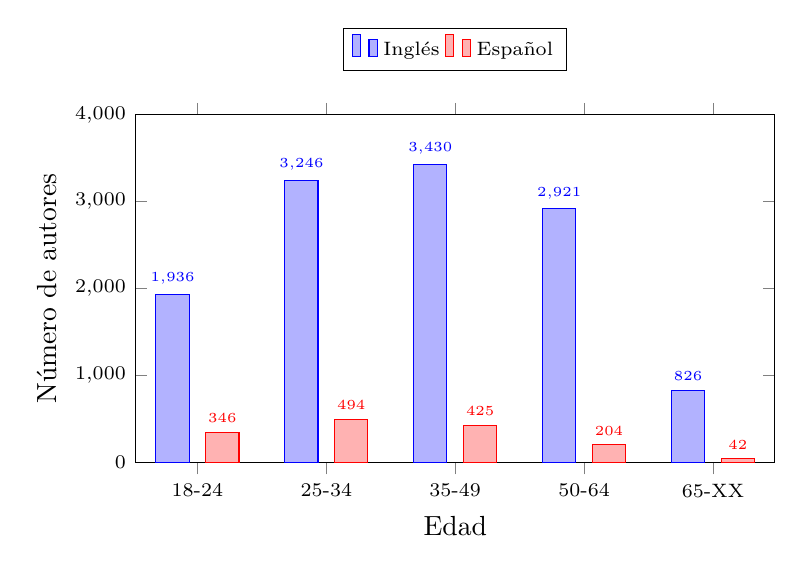
\begin{tikzpicture}
			\begin{axis}[
					width=0.8\textwidth,
					height=6cm,
					xmajorgrids=false,
					x tick label style={/pgf/number format/1000 sep=},
					x tick label style={font=\scriptsize},
					y tick label style={font=\scriptsize},
					ylabel=Número de autores,
					xlabel=Edad,
					ybar=6pt,
					bar width=12pt,
					enlarge x limits=0.12,
					nodes near coords,
					nodes near coords style={font=\tiny},
					symbolic x coords={18-24, 25-34, 35-49, 50-64, 65-XX},
					xtick=data,
					ymin=0,
					ymax=4000,
					legend style={at={(0.5,1.25)},font=\scriptsize, anchor=north,legend columns=-1},
			]
			\addplot table[x=Edad,y=Inglés] {
					Edad    Inglés
					18-24   1936
					25-34   3246
					35-49   3430
					50-64   2921
					65-XX   826
			};
			\addplot table[x=Edad,y=Español] {
					Edad    Español
					18-24   346
					25-34   494
					35-49   425
					50-64   204
					65-XX   42
			};
			\legend{Inglés, Español}
			\end{axis}
	\end{tikzpicture}
	\caption{Comparativa del número de autores por idioma en el \textit{corpus} del \textit{PAN Author Profiling 2014}}
	\label{fig:dataset_2014}
\end{figure}

\bigskip
\begin{table}[H]
	\centering
	\resizebox{0.7\textwidth}{!}{
		\rowcolors{2}{white}{udcgray!25}
		\begin{tabular}{|c|c|c|c|c|}
			\hhline{~|----|}
			\multicolumn{1}{c|}{\cellcolor{white}} & \multicolumn{2}{c|}{\cellcolor{udcpink!25}\textbf{Entrenamiento}} & \multicolumn{2}{c|}{\cellcolor{udcpink!25}\textbf{Test}} \\ \hline
			\textbf{Edad} & \textbf{Inglés} & \textbf{Español} & \textbf{Inglés} & \textbf{Español} \\ \hline
			18-24 & 1,936 & 346 & 850 & 158  \\ \hline
			25-34 & 3,246 & 494 & 1,380 & 218  \\ \hline
			35-49 & 3,430 & 425 & 1,470  & 210 \\ \hline
			50-64 & 2,921 & 204 & 1,226 & 92 \\ \hline
			65-XX & 826 & 42 & 324 & 32 \\ \hline
			\textbf{Total} & \textbf{12,359} & \textbf{1,511} & \textbf{5,250} & \textbf{710} \\ \hline
		\end{tabular}
	}
	\caption{Distribución del número de autores en cada rango de edad en el \textit{corpus} del \textit{PAN Author Profiling 2014}}
	\label{tab:dataset_2014}
\end{table}

\subsubsection{\textit{Resultados}}

Basándonos en los resultados de la competición, reflejados en la Tabla \ref{tab:algoritmos_2014}, podemos observar que los mejores datos de precisión
en cuanto a género fueron de alrededor de un 60\% para ambos idiomas, mientras que para la edad fueron de aproximadamente un 40\% para el inglés y de
un 50\% para el español.

\bigskip
En cuanto a las aproximaciones algorítmicas llevadas a cabo por los equipos mejor clasificados en la competición, podemos destacar lo siguiente:

\begin{itemize}
	\item \textbf{Preprocesado}: En cuanto al preprocesado, tanto Maharjan et al. \cite{maharjan2014simple} como Weren et al. \cite{weren2014exploring} realizaron un limpiado de los documentos XML para obtener
	texto plano, escapando caracteres inválidos en el caso del segundo equipo.
	\item \textbf{\textit{Features}}: En relación a las características extraídas de los documentos para la clasificación, Maharjan \cite{maharjan2014simple}, Weren et al. \cite{weren2014exploring} y Siang et al.,
	consideraron diferentes rasgos estilométricos como la frecuencia de los signos de puntuación, el tamaño de las frases o la frecuencia de las palabras, entre otros. Con respecto 
	a los rasgos basados en el contenido, Siang et al. y Maharjan et al. \cite{maharjan2014simple}, modelizaron el lenguaje con \textit{bag-of-word} y n-gramas, respectivamente, mientras
	que López-Monroy et al. \cite{lopez2014using} emplearon representaciones más complejas basadas en las relaciones entre palabras y documentos, explicadas a fondo
	en su trabajo.
	\item \textbf{Clasificación}: En cuanto a los algoritmos de clasificación utilizados, todos los equipos que aparecen en la Tabla \ref{tab:algoritmos_2014} emplearon regresión logística. López-Monroy et al. \cite{lopez2014using}
	hizo uso, más concretamente, de una librería de regresión logística y de SVMs lineales llamada LIBLINEAR (\textit{Large Linear Classification}) \cite{fan2008liblinear}.
\end{itemize}

\bigskip
\begin{table}[H]
	\centering
	\resizebox{0.9\textwidth}{!}{
		\rowcolors{2}{white}{udcgray!25}
		\setlength{\tabcolsep}{7pt}
		\begin{tabular}{|c|c|c|c|c|c|c|c|}
			\hhline{~|-------|}
			\multicolumn{1}{c|}{\cellcolor{white}} & \multicolumn{7}{c|}{\cellcolor{udcpink!25}\textbf{Precisión}} \\
			\hhline{~|-------|}
			\multicolumn{1}{c|}{\cellcolor{white}} & \multicolumn{3}{c|}{\textbf{Global}}  & \multicolumn{2}{c|}{\textbf{Inglés}} & \multicolumn{2}{c|}{\textbf{Español}} \\ \hline
			\textbf{Equipo participante} & \textbf{Conjunta} & \textbf{Género} & \textbf{Edad} & \textbf{Género} & \textbf{Edad} & \textbf{Género} & \textbf{Edad} \\ \hline
			López-Monroy et al. 2014 \cite{lopez2014using} & 0.2790 & 0.6310 & 0.4421 & 0.6512  & 0.3950 & 0.6108 & 0.4892 \\ \hline
			Siang et al. & 0.2758 & 0.6344 & 0.4348 & 0.663 & 0.3909 & 0.6057 & 0.4786 \\ \hline
			Maharjan et al., 2014 \cite{maharjan2014simple} & 0.2624 & 0.5948 & 0.4411 & 0.6132 & 0.3811 & 0.5764 & 0.5010 \\ \hline
			Weren et al., 2014 \cite{weren2014exploring} & 0.2266 & 0.5866 & 0.3863 & 0.6066 & 0.3690 & 0.5666 & 0.4035 \\ \hline
		\end{tabular}
	}
	\caption{Cuatro mejores clasificados en la competición \textit{PAN Author Profiling 2014}}
	\label{tab:algoritmos_2014}
\end{table}

\subsection{\textit{PAN Author Profiling 2015}}

En esta competición, a mayores de la clasificación por género y edad del autor, se añadió la predicción de rasgos de la personalidad. En concreto,
se buscaba predecir los cinco rasgos descritos en el modelo \textit{Big Five} (Goldberg, 1990) \cite{goldberg1990alternative}: extroversión (\textit{extroversion}),
estabilidad emocional / neuroticismo (\textit{stability / neuroticism}), apertura a la experiencia (\textit{openness to experience}), amabilidad (\textit{agreeableness}) y
responsabilidad (\textit{conscientiousness}). En cuanto a la edad, y a diferencia de la edición anterior de 2014, se eliminó la categoría de 65 años o más,
resultando en cuatro categorías: 18-24, 25-34, 35-49 y 50-XX.

\subsubsection{\textit{Corpus}}

\bigskip
En lo que respecta al \textit{corpus} proporcionado para la competición, los organizadores recopilaron \textit{tweets} de la red social Twitter
de 726 usuarios en cuatro idiomas diferentes: inglés, español, italiano y holandés. Dicho \textit{dataset} está etiquetado con el género y la edad
(solamente para inglés y español) de los autores, que ellos mismos reportaron en sus perfiles de Twitter. Para determinar los rasgos de la personalidad,
los autores completaron el test BFI-10 (Rammstedt et al., 2007) \cite{rammstedt2007measuring}, proporcionando valores para cada rasgo normalizados entre -0.5 y 0.5.

\bigskip
Así, como se puede ver en la Figura \ref{fig:dataset_2015}, el \textit{dataset} vuelve a estar desbalanceado en cuanto a la edad, ya que existen
clases como la 50-XX la cual apenas tiene un 7\% de la representación con respecto al total. Sin embargo,
a excepción de la clase 18-24, existe un número similar de autores de habla española e inglesa, por lo que cabe esperar una generalización
similar para ambos idiomas. En lo referente a la ditribución de género, como se puede ver en la Tabla \ref{tab:dataset_2015}, está perfectamente balanceada,
contando con un 50\% de autores de cada género para todos los idiomas.

\bigskip
\begin{figure}[H]
	\centering
	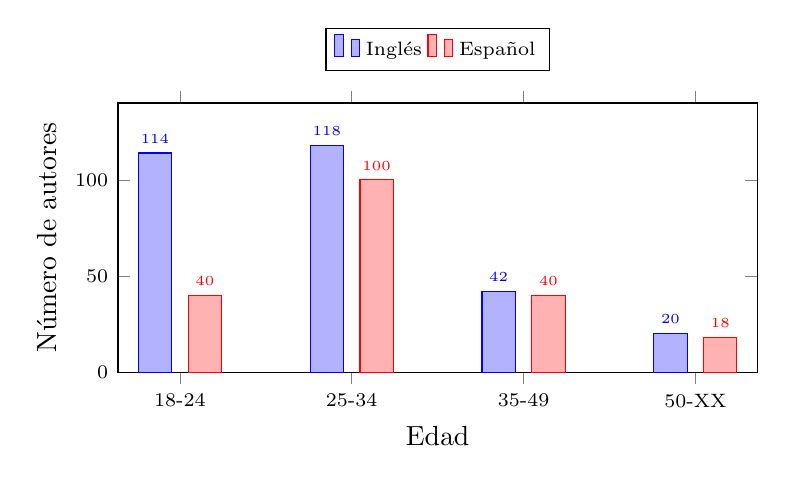
\begin{tikzpicture}
			\begin{axis}[
					width=0.8\textwidth,
					height=5cm,
					xmajorgrids=false,
					x tick label style={/pgf/number format/1000 sep=},
					x tick label style={font=\scriptsize},
					y tick label style={font=\scriptsize},
					ylabel=Número de autores,
					xlabel=Edad,
					ybar=6pt,
					bar width=12pt,
					enlarge x limits=0.12,
					nodes near coords,
					nodes near coords style={font=\tiny},
					symbolic x coords={18-24, 25-34, 35-49, 50-XX},
					xtick=data,
					ymin=0,
					ymax=140,
					legend style={at={(0.5,1.28)},font=\scriptsize, anchor=north,legend columns=-1},
			]
			\addplot table[x=Edad,y=Inglés] {
					Edad    Inglés
					18-24   114
					25-34   118
					35-49   42
					50-XX   20
			};
			\addplot table[x=Edad,y=Español] {
					Edad    Español
					18-24   40
					25-34   100
					35-49   40
					50-XX   18
			};
			\legend{Inglés, Español}
			\end{axis}
	\end{tikzpicture}
	\caption{Comparativa del número de autores por idioma en el \textit{corpus} del \textit{PAN Author Profiling 2015}}
	\label{fig:dataset_2015}
\end{figure}

\bigskip
\begin{table}[H]
	\centering
	\resizebox{0.9\textwidth}{!}{
		\rowcolors{2}{white}{udcgray!25}
		\setlength{\tabcolsep}{8pt}
		\begin{tabular}{|c|c|c|c|c|c|c|c|c|}
			\hhline{~|--------|}
			\multicolumn{1}{c|}{\cellcolor{white}} & \multicolumn{4}{c|}{\cellcolor{udcpink!25}\textbf{Entrenamiento}} & \multicolumn{4}{c|}{\cellcolor{udcpink!25}\textbf{Test}} \\ \hline
			\textbf{Característica} & \textbf{Inglés} & \textbf{Español} & \textbf{Italiano} & \textbf{Holandés} & \textbf{Inglés} & \textbf{Español} & \textbf{Italiano} & \textbf{Holandés} \\ \hline
			18-24 & 58 & 22 & - & - & 56 & 18 & - & -  \\ \hline
			25-34 & 60 & 56 & - & - & 58 & 44 & - & - \\ \hline
			35-49 & 22 & 22 & - & - & 20  & 18 & - & - \\ \hline
			50-XX & 12 & 10 & - & - & 8 & 8 & - & - \\ \hline
			\hline
			Masculino & 76 & 55 & 19 & 17 & 71 & 44 & 18 & 16 \\ \hline
			Femenino & 76 & 55 & 19 & 17 & 71 & 44 & 18 & 16 \\ \hline
			\hline
			Extrovertido & 0.16 & 0.18 & 0.17 & 0.24 & 0.17 & 0.16 & 0.15 & 0.24 \\ \hline
			Estabilidad & 0.14 & 0.07 & 0.20 & 0.21 & 0.13 & 0.09 & 0.20 & 0.22 \\ \hline
			Amabilidad & 0.12 & 0.14 & 0.22 & 0.13 & 0.14 & 0.14 & 0.19 & 0.15 \\ \hline
			Responsabilidad & 0.17  & 0.24 & 0.18 & 0.14 & 0.17 & 0.21 & 0.21 & 0.17 \\ \hline
			Apertura & 0.24 & 0.18 & 0.23 & 0.29 & 0.26 & 0.19 & 0.25 & 0.28 \\ \hline
		\end{tabular}
	}
	\caption{Distribución de los autores por característica y lenguaje en el \textit{corpus} del \textit{PAN Author Profiling 2015}}
	\label{tab:dataset_2015}
\end{table}

\subsubsection{\textit{Resultados}}

A la vista de los datos de precisión obtenidos por los primeros equipos clasificados, mostrados en la Tabla \ref{tab:algoritmos_2015},
podemos determinar que existe una gran mejora con respecto a los resultados de la competición anterior del año 2014, mejorando
la clasificación conjunta de edad y género en aproximadamente un 40\%.

\bigskip
Más en concreto, destacar los grandes resultados que
ofrecen los algoritmos presentados con respecto al género en los dos idiomas principales del \textit{corpus}, llegando a alcanzar
precisiones del 96\% para el español en el caso de Alvarez-Carmona et al. \cite{alvarez2015inaoe}. Con respecto a la edad,
se puede ver como se obtienen unos mejores resultados, de alrededor de un 5\%, en la clasificación en inglés que en español, algo que
hipotéticamente puede ser un reflejo de las pequeñas diferencias existentes entre el número de autores en cada uno de los idiomas en
el \textit{dataset} de entrenamiento.

\bigskip
Con respecto a la implementación de los algoritmos, podemos destacar lo siguiente:

\begin{itemize}
	\item \textbf{Preprocesado}: De forma similar a los algoritmos de años anteriores, la mayoría realizaron una limpieza del HTML incluído
	en los \textit{tweets} y, tanto González-Gallardo et al. \cite{gonzalez2015tweets} como Grivas et al. \cite{grivas2015author}, utilizaron
	las menciones, los \textit{hashtags} y los enlaces como características adicionales.
	\item \textbf{\textit{Features}}: En la mayor parte de los algoritmos presentados, se combinaba el uso de características
	basadas en el estilo y en el contenido. Así, en cuanto a contenido, González-Gallardo et al. \cite{gonzalez2015tweets} hizo uso de n-gramas de caracteres
	mientras que Grivas et al. \cite{grivas2015author} empleó n-gramas basados en TF-IDF. Además, en el caso de Grivas et al. \cite{grivas2015author},
	se analizaron otras caracterísitcas basadas en el estilo como la longitud de las palabras o el número de mayúsculas. En el caso de Alvarez-Carmona et al. \cite{alvarez2015inaoe},
	se hizo uso del Análisis Semántico Latente, explicado en la Sección \ref{sec:analisis_semantico_latente}, junto a una técnica similar a la empleada por
	López-Monroy et al. \cite{lopez2014using} en el año 2014.
	\item \textbf{Clasificación}: En lo referente a los métodos utilizados para realizar las predicciones, destaca el uso de la librería LIBLINEAR \cite{fan2008liblinear}
	por parte de Alvarez-Carmona et al. \cite{alvarez2015inaoe} y González-Gallardo et al. \cite{gonzalez2015tweets}. En el caso de Grivas et al. \cite{grivas2015author}, se hizo
	uso de SVMs para la clasificación del género y la edad mientras que se emplearon SVRs (Drucker et al., 1996) \cite{drucker1996support} para el reconocimiento de los rasgos personales.
\end{itemize}

\begin{table}[H]
	\centering
	\resizebox{\textwidth}{!}{
		\rowcolors{2}{white}{udcgray!25}
		\setlength{\tabcolsep}{6pt}
		\begin{tabular}{|c|c|c|c|c|c|c|c|c|c|}
			\hhline{~|---------|}
			\multicolumn{1}{c|}{\cellcolor{white}} & \multicolumn{9}{c|}{\cellcolor{udcpink!25}\textbf{Precisión}} \\
			\hhline{~|---------|}
			\multicolumn{1}{c|}{\cellcolor{white}} & \multicolumn{3}{c|}{\textbf{Global}} & \multicolumn{2}{c|}{\textbf{Inglés}} & \multicolumn{2}{c|}{\textbf{Español}} & \multicolumn{1}{c|}{\textbf{Italiano}} & \multicolumn{1}{c|}{\textbf{Holandés}} \\ \hline
			\textbf{Equipo participante} & \textbf{Conjunta} & \textbf{Género} & \textbf{Edad} & \textbf{Género} & \textbf{Edad} & \textbf{Género} & \textbf{Edad} & \textbf{Género} & \textbf{Género} \\ \hline
			Alvarez-Carmona et al. 2015 \cite{alvarez2015inaoe} & 0.7116 & 0.8712 & 0.8168 & 0.8592 & 0.8380 & 0.9659 & 0.7955 & 0.7222 & 0.9375 \\ \hline
			González-Gallardo et al., 2015 \cite{gonzalez2015tweets} & 0.6693 & 0.8871 & 0.7545 & 0.8521 & 0.7817 & 0.8977 & 0.7273 & 0.8611 & 0.9375 \\ \hline
			Grivas et al., 2015 \cite{grivas2015author} & 0.6487 & 0.9011 & 0.7199 & 0.8592 & 0.7465 & 0.9432 & 0.6932 & 0.8333 & 0.9688 \\ \hline
			Kocher et al., 2015 \cite{kocher2015unine} & 0.5655 & 0.7800 & 0.7250 & 0.7113 & 0.7113 & 0.8182 & 0.7386 & 0.7778 & 0.8125 \\ \hline
		\end{tabular}
	}
	\caption{Cuatro mejores clasificados en la competición \textit{PAN Author Profiling 2015}}
	\label{tab:algoritmos_2015}
\end{table}

\subsection{\textit{PAN Celebrity Profiling 2019}}

En esta última competición, la primera de ellas celebrada específicamente para el perfilado de celebridades, la tarea consistía en predecir
cuatro caracterísitcas demográficas a partir de sus publicaciones en Twitter:

\begin{itemize}
	\item \textbf{Género}: Masculino, femenino o no binario.
	\item \textbf{Año de nacimiento}: A la hora de calcular la precisión del algoritmos,
		se contemplará una ventana de error adaptativa entre los 2 y los 9 años en función de la edad real de la celebridad. 
	\item \textbf{Ocupación o motivo de fama}: Deportista (\textit{sports}), actor (\textit{performer}), político (\textit{politics}), creador de contenido (\textit{creator}),
		director (\textit{manager}), científico (\textit{science}), professional (\textit{professional}) o religioso (\textit{religious}).
	\item \textbf{Fama}: Revelación (\textit{rising}), estrella (\textit{star}) o superestrella (\textit{superstar}).
\end{itemize}

\subsubsection{\textit{Corpus}}

En este caso, como se mencionó anteriormente, el \textit{corpus} empleado está compuesto por publicaciones en inglés en la red social Twitter. En concreto,
el \textit{dataset} contenía un total de 48.335 celebridades con aproximadamente 2.180 \textit{tweets} cada una. El \textit{corpus} fue obtenido
a partir del \textit{Webis Celebrity Profiling Corpus} (Wiegmann et al., 2019) \cite{wiegmann2019celebrity}, en el cual se relacionaban los perfiles
de Twitter de las celebridades con sus entradas en Wikidata. De esta forma, se obtuvieron los \textit{tweets} de sus \textit{timelines} de la red social
y se simplificaron las caracterísitcas demográficas que ofrecía Wikidata, filtrando finalmente las celebridades nacidas antes de 1940 y que no tuvieran
el inglés como lengua de uso principal.

\bigskip
\begin{figure}[H]
	\centering
	\begin{subfigure}{0.5\textwidth}
			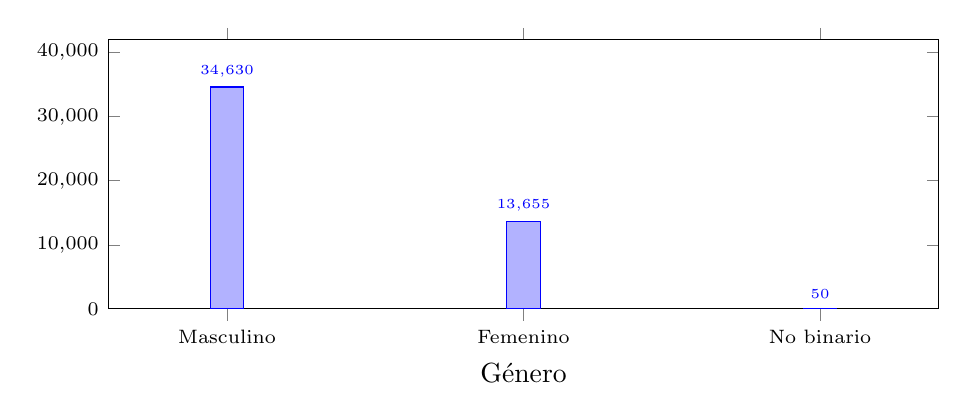
\begin{tikzpicture}
					\begin{axis}[
							width=\linewidth,
							height=5cm,
							xmajorgrids=false,
							x tick label style={font=\scriptsize},
							y tick label style={font=\scriptsize},
							ybar=6pt,
							bar width=12pt,
							enlarge x limits=0.2,
							ymin=0,
							ymax=42000,
							nodes near coords,
							nodes near coords style={font=\tiny},
							xtick=data,
							xticklabels={Masculino, Femenino, {No binario}},
							xlabel={Género},
							scaled y ticks=false
					]
					\addplot coordinates {(1,34630) (2,13655) (3,50)};
					\end{axis}
			\end{tikzpicture}
			\label{fig:distribucion_genero_2019}
	\end{subfigure}%
	\hfill
	\begin{subfigure}{0.5\textwidth}
			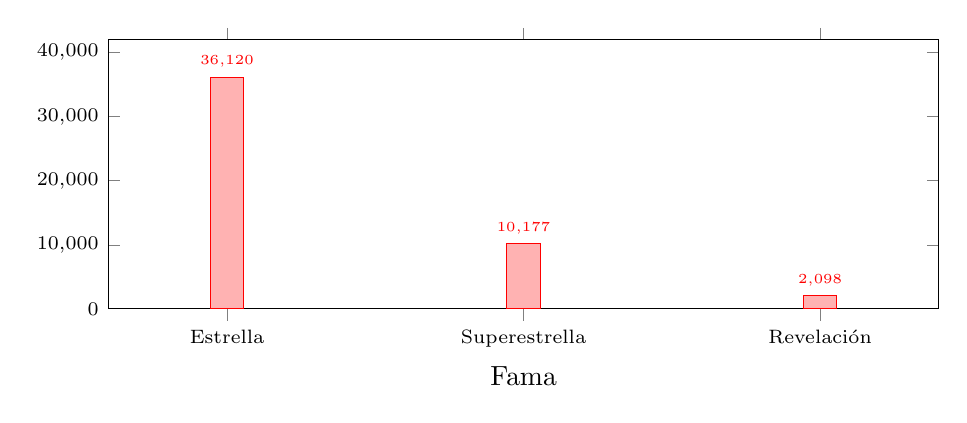
\begin{tikzpicture}
					\begin{axis}[
							width=\linewidth,
							height=5cm,
							xmajorgrids=false,
							x tick label style={font=\scriptsize},
							y tick label style={font=\scriptsize},
							ybar=6pt,
							bar width=12pt,
							enlarge x limits=0.2,
							ymin=0,
							ymax=42000,
							nodes near coords,
							nodes near coords style={font=\tiny},
							xtick=data,
							xticklabels={Estrella, Superestrella, Revelación},
							xlabel={Fama},
							scaled y ticks=false
					]
					\addplot[color=red, fill=red!30] coordinates {(1,36120) (2,10177) (3,2098)};
					\end{axis}
			\end{tikzpicture}
			\label{fig:distribucion_fama_2019}
	\end{subfigure}
	\caption{Distribuciones de género y fama en el \textit{corpus} de la competición \textit{PAN Celebrity Profiling 2019}.}
	\label{fig:distribuciones_2019}
\end{figure}

\begin{figure}[H]
	\centering
	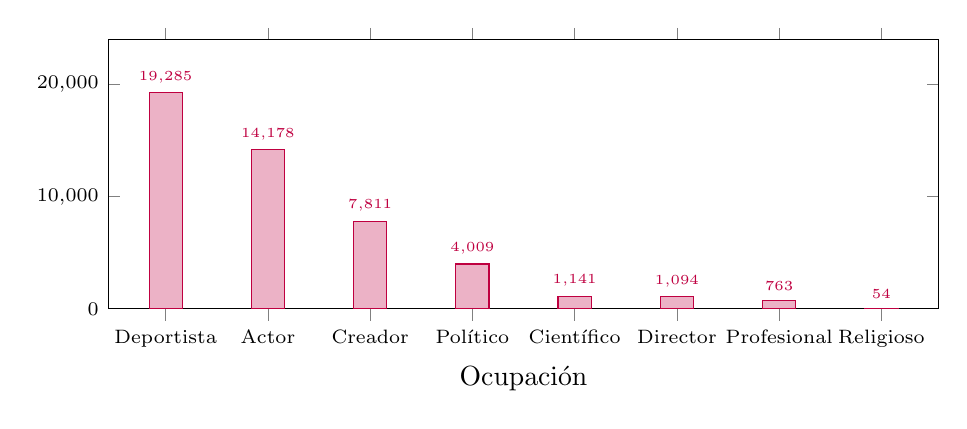
\begin{tikzpicture}
		\begin{axis}[
				width=\linewidth,
				height=5cm,
				xmajorgrids=false,
				x tick label style={font=\scriptsize},
				y tick label style={font=\scriptsize},
				ybar=6pt,
				bar width=12pt,
				enlarge x limits=0.08,
				ymin=0,
				ymax=24000,
				nodes near coords,
				nodes near coords style={font=\tiny},
				xtick=data,
				xticklabels={Deportista, Actor, Creador, Político, Científico, Director, Profesional, Religioso},
				xlabel={Ocupación},
				scaled y ticks=false
		]
		\addplot[color=purple, fill=purple!30] coordinates {(1,19285) (2,14178) (3,7811) (4,4009) (5,1141) (6,1094) (7,763) (8,54)};
		\end{axis}
	\end{tikzpicture}
	\label{fig:distribucion_ocupacion_2019}
	\caption{Distribución de ocupaciones en el \textit{corpus} de la competición \textit{PAN Celebrity Profiling 2019}.}
\end{figure}

\begin{table}[H]
	\centering
	\resizebox{0.8\textwidth}{!}{
		\rowcolors{2}{white}{udcgray!25}
		\begin{tabular}{|c|c|c|c|}
			\hhline{~|---|}
			\multicolumn{1}{c|}{\cellcolor{white}} & \multicolumn{3}{c|}{\cellcolor{udcpink!25}\textbf{Precisión}} \\ \hline
			\textbf{Equipo participante} & \textbf{Conjunta} & \textbf{Género} & \textbf{Edad} \\ \hline
			Radivchev et al. 2019 \cite{radivchev2019celebrity} & 0.477 & 0.928 & 0.514  \\ \hline
			Martinc et al., 2019 \cite{martinc2019hot} & 0.410 & 0.906 & 0.453 \\ \hline
			Fernquist et al., 2019 & 0.362 & 0.774 & 0.468 \\ \hline
			Moreno-Sandoval et al., 2019 \cite{moreno2019celebrity} & 0.320 & 0.862 & 0.371  \\ \hline
		\end{tabular}
	}
	\caption{Cuatro mejores clasificados en la competición \textit{PAN Celebrity Profiling 2019}}
	\label{tab:algoritmos_2019}
\end{table}

\subsection{Martinc}
\label{sec:algoritmos_martinc}

\subsection{Grivas}
\label{sec:algoritmos_grivas}

\chapter{Herramientas, técnicas y lenguajes}
\label{chap:herramientas}

Para estructurar mejor todas las herramientas y tecnologías utilizadas en el desarrollo de este proyecto, se han dividido en tres secciones:
\begin{itemize}
		\item Backend \ref{sec:herramientas_backend}: Sección en la que se explican las herramientas utilizadas para la programación del servidor y de la API REST.
		\item Frontend \ref{sec:herramientas_frontend}: Sección en la que se explican las herramientas utilizadas para la programación de la interfaz de visualización.
		\item Algoritmos de perfilado \ref{sec:herramientas_algoritmos}: Sección en la que se explican las herramientas utilizadas para la ejecución de los algoritmos de perfilado.
\end{itemize}
	
\section{\textit{Backend}}
\label{sec:herramientas_backend}

Ya que para el \textit{backend} no se necesitaba nada excesivamente complejo, se decidió utilizar el lenguaje de programación Python \cite{python} junto
con el \textit{framework} FastAPI \cite{fastapi}, el cual permite crear APIs REST de forma sencilla. La decisión de utilizar Python, viene también
condicionada por el hecho de que los algoritmos de perfilado de autor utilizados, así como también la mayor parte de los algoritmos de aprendizaje automático, 
están ya programados en Python, evitando así crear nuevos \textit{endpoints}, \textit{sockets} o \textit{bindings} para la ejecución de dichos algoritmos.
Destacar también que el desarrollo ágil en Python favorecía mucho al trabajo debido a su tipado dinámico, a su ejecución interpretada y a su sintaxis sencilla.

\bigskip
Por otro lado, para que el cógido estuviese bien organizado, se decidió utilizar el patrón de diseño DDD (del inglés \textit{Domain-Driven Design}) \cite{ddd}, el cual
permite separar el código en tres capas: la capa de aplicación, la capa de dominio y la capa de infraestructura. La capa de aplicación es la encargada de gestionar
la entrada y salida de la aplicación que, en nuestro caso, es el controlador que maneja los \textit{endpoints} REST; la capa de dominio es la que contiene la lógica
de negocio y las entidades; y la capa de infraestructura es la responsable de administrar las interacciones internas de la aplicación que, en nuestro
caso, se encarga de la comunicación con la base de datos.

\bigskip
Esta es una figura adaptada de https://www.baeldung.com/hexagonal-architecture-ddd-spring Łukasz Ryś 2022
\begin{figure}[H]
	\centering
	\includegraphics[width=0.9\textwidth]{diagramas/ddd.pdf}
	\caption{Diagrama de capas del patrón de diseño DDD}
	\label{fig:ddd}
\end{figure}

\section{\textit{Frontend}}
\label{sec:herramientas_frontend}

En cuanto al \textit{frontend}, se decidió utilizar NextJS \cite{nextjs} como herramienta para el desarrollo de la interfaz de usuario, dado que ya
se contaba con bastante experiencia previa en su uso. NextJS es un \textit{framework} basado en React \cite{react}, es decir, en la construcción de interfaces dinámicas mediante la composición
de elementos que pueden tener estado. Además, este \textit{framework} implementa varias mejoras sobre React como por ejemplo el \textit{server-side rendering}, algo que ayuda en gran medida
al SEO (del inglés \textit{Search Engine Optimizations}), es decir, a que los motores de búsqueda como Google puedan indexar mejor la página y, por tanto, que esta aparezca en una posición superior en los resultados de búsqueda.
Además, también cuenta con optimizaciones para la carga y el renderizado de imágenes o fuentes entre otras.

\bigskip
Todo ello se desarrolló utilizando TypeScript \cite{typescript}, un lenguaje de programación que añade tipado estático a JavaScript
y que está ganando mucha popularidad con respecto a la mentinibilidad, compresión y escalabilidad que proporciona a los proyectos en los que se usa (Stack Overflow, 2023) \cite{stackoverflow2023}.

\bigskip
En cuanto el estilado de la página, se optó por emplear SASS (del inglés \textit{Syntactically Awesome Style Sheets}) \cite{sass}, un preprocesador de CSS (del inglés \textit{Cascading Style Sheets}) que añade
funcionalidades extra como son el uso de variables, bucles o anidamiento de clases. Además, dado que se estaba desarrollando
una aplicación novedosa, se buscó crear un estilo propio haciendo uso de CSS "nativo", desmarcándose así de librerías que proporcionasen estilos predefinidos como Bootstrap \cite{bootstrap} o componentes ya implementados
como Material UI \cite{materialui} o Chakra UI \cite{chakraui}. Por otra parte, para la creación de gráficos se utilizó la librería ChartJS \cite{chartjs}, una de las más conocidas
y con más soporte en la actualidad. Finalmente, para implementar las animaciones en la interfaz, se hizo uso, en conjunto con las transiciones nativas
de CSS, de Framer Motion \cite{framermotion}, una librería que permite crear animaciones más complejas desde JavaScript/TypeScript. 

\section{Algoritmos de perfilado}
\label{sec:herramientas_algoritmos}

\section{Soporte}

\chapter{Metodología}
\label{chap:metodologia}

Para el desarrollo de este proyecto se ha utilizado una metodología ágil, concretamente Scrum \cite{scrum}.
Esta metodología se basa en la realización de iteraciones cortas, llamadas \textit{sprints}, en las que se desarrolla una parte del proyecto
denominada incrementeo, es decir, una versión entregrable del producto que contiene
nuevas funcionalidades o mejoras de las ya existentes. La decisión de optar por una metodología de tipo ágil frente a una tradicional
está condicionada por el tiempo de desarrollo corto, de apenas cuatro meses, y por los cambios que se podían producir en los requisitos.
Además, todo el equipo se sentía más cómodo con esta metodología dado que ya se tenía experiencia anterior en su uso.

\section{Roles}
\label{sec:metodologia_roles}

En Scrum existen tres roles principales:

\begin{itemize}
		\item \textbf{Product Owner}: Como su nombre indica, es el propietario del producto, por lo que es el encargado de identificar
		las necesidades de los clientes así como de definir y gestionar el \textit{Product Backlog}, esto es, la lista de requisitos del producto ordenados por prioridad.
		Este rol es desempeñado por el autor de este documento.
		\item \textbf{Scrum Master}: Su rol principal es el de asegurar que el equipo de desarrollo sigue la metodología Scrum y no se producen
		desajustes en el transcurso del proyecto. Los encargados de asumir este rol fueron Patricia Martín Rodilla y David Otero Freijeiro, los
		tutores de este trabajo.
		\item \textbf{Equipo de desarrollo}: Formado por un equipo normalmente de entre tres y nueve personas, es el encargado de desarrollar el producto
		en cada \textit{sprint} cumpliendo los requisitos establecidos en el \textit{Product Backlog}. En este caso, el equipo de desarrollo está
		formado únicamente por el autor de este documento.
\end{itemize}

\section{Eventos}
\label{sec:metodologia_eventos}

Para agilizar el desarrollo y no interferir en el trabajo diario del equipo por las obligaciones
externas de cada uno, tanto las reuniones de planificación como las de revisión y retrospectiva se realizan
el mismo día que se inicia cada \textit{sprint}, esto es, aproximadamente cada tres semanas, lo que se ajusta a la duración recomendada
por la metodología Scrum. Estas reuniones son, por lo tanto, de una mayor extensión que las \textit{dailies} clásicas y son también empleadas
para realizar una revisión del incremento desarrollado en el úlitmo \textit{sprint}.

\chapter{Análisis}
\label{chap:analisis}

\lettrine{E}{n} este capítulo se expondrán los requisitos obtenidos tras el estudio de las necesidades que debe cubrir la aplicación
y se elaborarán las historias de usuario.

\section{Requisitos funcionales}
\label{sec:analisis_requisitos_funcionales}

Para la definición de los requisitos funcionales que debe cumplir la aplicación, se ha hecho uso de las historias de usuario.
Esta técnica permite definir los requisitos de una forma más cercana al usuario, ya que se centra en la descripción
de las funcionalidades que este desea que tenga el sistema. Con todo, tanto el diagrama de casos de uso para la interfaz
como las historias de usuario obtenidas se muestran en la Figura \ref{fig:casos_uso} y la Tabla \ref{tab:historias_usuario}, respectivamente.

\bigskip
\begin{figure}[H]
	\centering
	\includegraphics[width=\textwidth]{diagramas/usecases.pdf}
	\caption{Diagrama de casos de uso para la interfaz de usuario}
	\label{fig:casos_uso}
\end{figure}

\bigskip
\begin{table}[H]
	\centering
	\rowcolors{2}{white}{udcgray!25}
	\begin{tabular}{|c|p{11cm}|}
		\rowcolor{udcpink!25}
		\hline
		\small \textbf{ID}                 & \small \textbf{Historia de usuario}                                                                      \\\hline
		\small \textbf{H1} \label{req:hu1} & \small Como usuario quiero poder subir mi propio \textit{dataset} de textos para su perfilado            \\ \hline
		\small \textbf{H2} \label{req:hu2} & \small Como usuario quiero conocer ejemplos del formato de los \textit{datasets} aceptados               \\ \hline
		\small \textbf{H3} \label{req:hu3} & \small Como usuario quiero poder seleccionar el algoritmo de perfilado que se va a utilizar              \\ \hline
		\small \textbf{H4} \label{req:hu4} & \small Como usuario quiero poder visualizar los datos obtenidos tras el perfilado                        \\ \hline
		\small \textbf{H5} \label{req:hu5} & \small Como usuario quiero poder ver una lista detallada de cada persona perfilada                       \\ \hline
		\small \textbf{H6} \label{req:hu6} & \small Como usuario quiero poder ordenar la lista de personas por cada uno de los campos perfilados      \\ \hline
		\small \textbf{H7} \label{req:hu7} & \small Como usuario quiero poder saber como funcionan los diferentes algoritmos de perfilado disponibles \\ \hline
		\small \textbf{H8} \label{req:hu8} & \small Como usuario quiero ver el rendimiento de los algoritmos de perfilado disponibles                 \\ \hline
		\small \textbf{H9} \label{req:hu9} & \small Como usuario quiero poder reentrenar los algoritmos con diferentes \textit{datasets}              \\ \hline
	\end{tabular}
	\caption{Historias de usuario de la aplicación}
	\label{tab:historias_usuario}
\end{table}

\newpage
\section{Requisitos no funcionales}
\label{sec:analisis_requisitos_no_funcionales}

Una vez definidas las funcionalidades que debe tener la aplicación, es necesario definir cuales van a ser sus requisitos
no funcionales, esto es, aquellos que están relacionados con cómo debe funcionar la aplicación. En este sentido, a pesar
de que la propia metodología Scrum no contempla la definición de requisitos no funcionales más allá de las historias de usuario,
se ha considerado adaptar esta parte y definirlos por separado para dotarlos de una mayor importancia.
De esta forma, se han determinado los requisitos recogidos en la Tabla \ref{tab:requisitos_no_funcionales}.

\bigskip
\begin{table}[hp!]
	\centering
	\rowcolors{2}{white}{udcgray!25}
	\begin{tabular}{|c|c|p{7.5cm}|}
		\rowcolor{udcpink!25}
		\hline
		\small \textbf{ID}                    & \small \textbf{Requisito} & \small \textbf{Descripción}                                                                      \\\hline
		\small \textbf{RNF1} \label{req:rnf1} & \small Usabilidad         & \small La aplicación debe ser fácil de usar, de forma que cualquier usuario pueda utilizarla sin
		necesidad de tener conocimientos previos sobre el perfilado de autores.                                                                                              \\\hline
		\small \textbf{RNF2} \label{req:rnf2} & \small Escalabilidad      & \small La aplicación debe ser capaz de procesar \textit{datasets} de cualquier tamaño.           \\\hline
		\small \textbf{RNF3} \label{req:rnf3} & \small Portabilidad       & \small La aplicación debe ser capaz de ejecutarse en cualquier sistema, haciendo que
		los usuarios no tengan que preocuparse por el dispositivo que utilizan.                                                                                              \\\hline
		\small \textbf{RNF4} \label{req:rnf4} & \small Extensibilidad     & \small La aplicación debe permitir una fácil extensión de sus funcionalidades, de forma que
		no afecte al funcionamiento de las ya existentes.                                                                                                                    \\\hline
	\end{tabular}
	\caption{Requisitos no funcionales}
	\label{tab:requisitos_no_funcionales}
\end{table}

\chapter{Diseño}
\label{chap:diseño}

Para abordar el diseño de la aplicación a lo largo de este capítulo, se detallará la arquitectura software elegida para el sistema
y se mostrarán los prototipos de la interfaz de usuario.

\section{Arquitectura}
\label{sec:diseño_arquitectura}

Teniendo en cuenta los requisitos definidos en las Secciones \ref{sec:analisis_requisitos_funcionales} y \ref{sec:analisis_requisitos_no_funcionales},
así como también las limitaciones temporales del proyecto, se ha optado por una arquitectura cliente-servidor. Esta aquitectura se ha elegido
por la facilidad en su implementación y por su capacidad de intercomunicación con otros sistemas, especialmente con clientes web. Como
se aprecia en la Figura \ref{fig:arquitectura_contenedor}, el servidor cuenta con un controlador REST capaz de redirigir las peticiones al servicio
corresepondiente. En este sentido, a pesar de solo contar con un único servicio (\textit{Servicio de perfilado}) en la versión actual,
la arquitectura cliente-servidor permite añadir nuevos servicios, junto a nuevas funcionalidades, de forma sencilla y sin poner en riesgo al resto del sistema.
Dicho servicio será el que se comunique con la base da datos para garantizar la persistencia de los datos del perfilado y permitir así
una posterior consulta.

\bigskip
Por otro lado, para que el código estuviese bien organizado, se decidió utilizar el patrón de diseño DDD (del inglés \textit{Domain-Driven Design}) \cite{ddd}, el cual
permite separar el código en tres capas: la capa de aplicación, la capa de dominio y la capa de infraestructura. La capa de aplicación es la encargada de gestionar
la entrada y salida de la aplicación que, en nuestro caso, es el controlador que maneja los \textit{endpoints} REST; la capa de dominio es la que contiene la lógica
de negocio y las entidades; y la capa de infraestructura es la responsable de administrar las interacciones internas de la aplicación que, en nuestro
caso, se encarga de la comunicación con la base de datos.

\begin{figure}[H]
	\centering
	\includegraphics[width=0.9\textwidth]{diagramas/ddd.pdf}
	\caption{Diagrama de capas del patrón de diseño DDD. Adaptado de Ł, Ryś \cite{dddblog}}
	\label{fig:ddd}
\end{figure}

\bigskip
A mayores, el propio \textit{frontend} web tendrá también una arquitecture basada en cliente-servidor, en la que el servidor será el encargado
de ofrecer al cliente los archivos estáticos necesarios para mostrar la interfaz (HTML, CSS, JavaScript, fuentes, imágenes...). El hecho
de elegir una interfaz web gira en torno al requisito no funcional de portabilidad definido en la Sección \ref{sec:analisis_requisitos_no_funcionales},
puesto que de esta forma, la aplicación podría ser utilizada por cualquier dispositivo con un navegador web, evitando
desarrollar aplicaciones nativas para cada sistema operativo.

\bigskip
\begin{figure}[H]
	\centering
	\includegraphics[width=0.7\textwidth]{diagramas/arquitectura_contenedor.pdf}
	\caption{Diagrama C4 de Contenedor de la arquitectura del sistema.}
	\label{fig:arquitectura_contenedor}
\end{figure}

\section{Prototipado}
\label{sec:diseño_prototipado}

Como se mencionó anteriormente, para el diseño de los prototipos de pantallas, también conocidos como \textit{wireframes}, se utilizó
la herramienta Draw.io \cite{drawio} debido a su sencillez y rapidez en la elaboración con respecto a otros programas más avanzados
como pueden ser Adobe XD \cite{adobexd} o Figma \cite{figma}.

\bigskip
La filosofía de diseño de la interfaz se centró en el minimalismo y la usabilidad, como se indica en la Sección \ref{sec:analisis_requisitos_no_funcionales}
, por lo que todo estará caracterizado por no contener excesivos elementos y por ser fácilmente comprensible para el usuario. 

\bigskip
La pantalla de inicio, como se ve en la Figura \ref{fig:prototipo_inicio}, está compuesta simplemente por un título, 
un subtítulo y un campo que permitirá al usuario subir un \textit{dataset}, tanto mediante un elemento \textit{drag and drop} como
mediante un botón que abrirá el explorador de archivos del sistema operativo.

\bigskip
\begin{figure}[H]
	\centering
	\includegraphics[width=\textwidth]{diagramas/landing.pdf}
	\caption{Prototipo de la pantalla de inicio}
	\label{fig:prototipo_inicio}
\end{figure}

\bigskip
Una vez el usuario haya subido el \textit{dataset}, el campo de subida se sustituirá por la lista de los
algoritmos de perfilado disponibles, como se puede ver en la Figura \ref{fig:prototipo_algoritmo_perfilado}. De cada algoritmo se mostrará, en una tarjeta, las características que es capaz de extraer
del perfilado junto con su título. Además, ya que uno de los requisitos era el de mostrar información del funcionamiento
y del rendimiento de los algoritmos, se decidió crear un \textit{tooltip} que se mostrase cada vez que el usuario pasase el ratón
por encima de cada tarjeta. Finalmente, si el usuario desease cambiar el \textit{dataset} seleccionado, se permitirá retroceder mediante
la flecha situada junto al título del paso actual.

\bigskip
\begin{figure}[H]
	\centering
	\includegraphics[width=\textwidth]{diagramas/landing-algorithm.pdf}
	\caption{Prototipo de la selección del algoritmo de perfilado}
	\label{fig:prototipo_algoritmo_perfilado}
\end{figure}

\bigskip
Ya con el \textit{dataset} y el algoritmo seleccionados, se presentará al usuario un resumen del perfilado, donde se mostrará
el nombre del fichero subido, la tarjeta del algoritmo seleccionado y un botón que permitirá al usuario comenzar con el proceso de perfialdo.
Además, como se aprecia en la Figura \ref{fig:prototipo_resumen_perfilado}, una vez comienza el perfilado, se mostrará una barra de progreso
o un \textit{spinner} que le indicará al usuario que el proceso está en marcha. De la misma forma que en el paso anterior, si el usuario
decide cambiar de algoritmo, puede retroceder haciendo uso de la flecha situada junto al título del paso actual.

\bigskip
\begin{figure}[H]
	\centering
	\includegraphics[width=\textwidth]{diagramas/landing-overview.pdf}
	\caption{Prototipo del resumen del perfilado}
	\label{fig:prototipo_resumen_perfilado}
\end{figure}

\bigskip
Con respecto a la pantalla de ejemplos de \textit{datasets}, como se puede ver en la Figura \ref{fig:prototipo_ejemplos_dataset},
se mostrará un pequeño ejemplo de 10-15 líneas aproximadamente. Asimismo, se le dará la opción al usuario de seleccionar el 
formato de \textit{dataset}, ya sea NDJSON o CSV, dado que son los que soportará el \textit{backend}.

\bigskip
\begin{figure}[H]
	\centering
	\includegraphics[width=\textwidth]{diagramas/dataset-examples.pdf}
	\caption{Prototipo de la pantalla de ejemplos de dataset}
	\label{fig:prototipo_ejemplos_dataset}
\end{figure}

\bigskip
Cuando el perfilado haya finalizado, se mostrará al usuario un \textit{dashboard} con los resultados obtenidos,
como se puede ver en las Figuras \ref{fig:prototipo_dashboard_martinc}, \ref{fig:prototipo_dashboard_grivas}. 
Este \textit{dashboard} contendrá los siguientes gráficos y elementos, los cuales variarán en función del algoritmo utilizado:

\begin{itemize}
	\item \textbf{Datos generales}: El \textit{dashboard} contiene una primera sección en la que aparece información de carácter general
		como son: el número total de personas perfiladas, el tiempo total del perfilado y el algoritmo utilizado.
	\item \textbf{Lista detallada de personas}: En esta sección, se muestra la lista de personas perfiladas de forma paginada. Además, la lista
		permitirá ser ordenada por cada uno de los diferentes campos, según se indica en la historia de usuario con identificador 
		\textit{6} de la Sección \ref{sec:analisis_requisitos_funcionales}. Para ello, el usuario deberá hacer clic en el nombre de dicho campo, teniendo
		la opción de, volviendo a clicar, cambiar el sentido de ordenación (ascendente o descendente).
	\item \textbf{Distribución de edad}: Para la distribución de edad, se ha optado por un gráfico de barras sobre otras opciones de representación
		categóricas como el gráfico circular. Esto se debe a que, teniendo cinco clases diferentes, el gráfico de barras permite una mejor visualización 
		de los datos y una comparativa más clara entre ellos, dado que es más fácil comparar longitudes que áreas o ángulos. En la parte inferior del gráfico,
		se mostrará una tarjeta con la edad mediana.
	\item \textbf{Distribución de género}: En cuanto a la distribución de género, en cambio, se ha optado por un gráfico circular, puesto que solo existen dos clases
		y se desea resaltar la proporción de cada clase con respecto al total. A mayores, se mostrarán debajo del gráfico dos tarjetas con el número de personas
		de cada género junto con su porcentaje exacto.
	\item \textbf{Distribución de fama \textit{(Martinc)}}: De forma similar a la distribución de género, solo contamos con tres clases diferentes, por lo que
		se ha elegido un gráfico circular. Resaltar que este gráfico solo se mostrará en el caso de que se haya utilizado el algoritmo de Martinc.
	\item \textbf{Distribución de ocupación \textit{(Martinc)}}: En el caso de la distribución de ocupación, debido a que existen ocho clases distintas, se ha optado
		por un gráfico de barras. Este gráfico, al igual que el anterior, solo aparecerá si se ha empleado el algoritmo de Martinc para el perfilado.
	\item \textbf{Características personales \textit{(Grivas)}}: Ya que en este caso cada característica personal tendría asociado un valor decimal entre -0.5 y 0.5,
		se ha optado por un gráfico de barras. En este sentido, cabe resaltar que para mostrar dicho gráfico, es necesario implementar una funcionalidad que permita
		seleccionar a una persona de la lista detallada para mostrar sus características personales. Además, este gráfico solo estará disponible si se hace uso del algoritmo de Grivas.
\end{itemize}

\bigskip
\begin{figure}[H]
	\centering
	\includegraphics[width=\textwidth]{diagramas/dashboard-martinc.pdf}
	\caption{Prototipo del dashboard utilizando el algoritmo Martinc}
	\label{fig:prototipo_dashboard_martinc}
\end{figure}

\bigskip
\begin{figure}[H]
	\centering
	\includegraphics[width=\textwidth]{diagramas/dashboard-grivas.pdf}
	\caption{Prototipo del dashboard utilizando el algoritmo Grivas}
	\label{fig:prototipo_dashboard_grivas}
\end{figure}

\chapter{Implementación}
\label{chap:implementacion}

\lettrine{A} lo largo de este capítulo, se expondrán las decisiones de implementación más relevantes tomadas durante el desarrollo de la aplicación.
y se detallará la estructura de directorios que se ha seguido para organizar el código fuente del proyecto. Finalmente, se hablará
de la importancia del código abierto y de como contribuye a la innovación en el campo de la informática.

\section{Adaptación de los algoritmos}
\label{sec:adaptacion_algoritmos}

Dado que el código fuente de los algoritmos de perfilado seleccionados estaba disponible para su uso, fue necesario adaptarlo
para ofrecer una interfaz común a través de la cual se pudiese comunicar el resto de la aplicación.
Para ello se barajaron en un inicio dos aproximaciones diferentes. La primera de ellas pasaba
por implementar APIs sencillas en cada uno de los algoritmos, es decir, crear microservicios que se encargasen de recibir
las peticiones y devolver los resultados al \textit{backend}. La segunda aproximación consistía en adaptar el propio código
fuente para que cada algoritmo formase parte de una clase que implemente la interfaz mencionada en el diagrama de la Figura \ref{fig:clases_backend}
(\textit{ProfilingAlgorithm}). Finalmente, se optó por esta segunda opción ya que, a pesar de ser más compleja, permitía
una mayor integración con el resto de la aplicación y un mejor rendimiento debido a la eliminación de la latencia de red. Además,
podíamos aprovechar el hecho de que los algoritmos estaban programados en Python para utilizarlos directamente
en el \textit{backend} sin hacer uso de llamadas interlenguaje.

\bigskip
Sin embargo, esta decisión implicó comprender a muy bajo nivel como estaban implementados dichos algoritmos para realizar las modificaciones necesarias
e implementar nuevas funciones. Esta adaptación del código fue, en el caso del algoritmo de Grivas et al. \cite{grivas2015author},
bastante compleja, ya que conllevó sustituir librerías obsoletas, reimplementar funciones y resolver los cambios disruptivos (\textit{breaking changes} en inglés) que suponía
dar el salto desde la versión 2.7 de Python a la 3.10.

\section{Estructura del proyecto}
\label{sec:estructura_proyecto}

En relación a la estructura del proyecto, se ha optado por agrupar el código fuente de todo el sistema
bajo un mismo directorio, como se muestra en el diagrama de la Figura \ref{fig:estructura_proyecto},
dado que facilita en gran medida su portabilidad y su mantenimiento al tratarse de un proyecto relativamente
pequeño.

\bigskip
En primer lugar, situados en la raíz del proyecto, podemos diferenciar las carpetas principales que lo conforman, esto es,
\textit{backend}, \textit{fronted} y \textit{datasets}, así como dos archivos:

\begin{itemize}
	\item \textbf{\textit{README.md}}: Contiene un resumen en formato Markdown \cite{markdown} de lo que es la aplicación, de sus características y de la forma de ejecutarla.
	\item \textbf{\textit{docker-compose.yml}}: Es el archivo que almacena las configuraciones de los contenedores de Docker que se deben levantar para que el sistema funcione adecuadamente.
\end{itemize}

\bigskip
Continuando con el directorio \textit{backend}, distinguimos varias carpetas y archivos:

\begin{itemize}
	\item \textbf{\textit{requirements.txt}}: Contiene todas las dependencias de Python que necesita el \textit{backend} para funcionar.
	\item \textbf{\textit{Dockerfile}}: Es el archivo en el que se definen los pasos necesarios, es decir, los comandos a ejecutar en una
	      máquina recién instalada, para construir la imagen de Docker del \textit{backend}.
	\item \textbf{\textit{docker-compose.yml}}: A diferencia del situado en la raíz, este archivo contiene las configuraciones de los contenedores necesarios
	      para el correcto funcionamiento del entorno de desarrollo en el \textit{backend}.
	\item \textbf{\textit{/venv}}: Dado que el proyecto está creado haciendo uso de un entorno virtual para aislar las dependencias de Python, este directorio
	      contiene los archivos para su puesta en marcha.
	\item \textbf{\textit{/src}}: Aquí se almacena todo el código fuente del \textit{backend}, donde podemos encontrar las siguientes carpetas principales:
	      \begin{itemize}
		      \item \textbf{\textit{/application}}: Contiene los controladores y, en general, lo que se encarga de gestionar las comunicaciones exteriores con el sistema.
		      \item \textbf{\textit{/domain}}: Contiene las clases que conforman la capa de dominio, es decir, las entidades, los repositorios, los servicios, los algoritmos
		            y los conversores.
		      \item \textbf{\textit{/infraestructure}}: Contiene los repositorios de tecnologías concretas que implementan las interfaces definidas en la capa de dominio.
		      \item \textbf{\textit{/utils}}: Contiene clases de utilidad requeridas en diversas partes del sistema.
		      \item \textbf{\textit{main.py}}: Se corresponde con el punto de entrada de la aplicación.
	      \end{itemize}
\end{itemize}

\bigskip
Por otro lado, la estructura que sigue el \textit{frontend}, muy ligada al \textit{framework} de desarrollo NextJS, es la siguiente:

\begin{itemize}
	\item \textbf{\textit{package.json}}: En este archivo se almacenan todas las dependencias de NodeJS que requiere el \textit{frontend}.
	\item \textbf{\textit{next.config.js}}: La importancia de este archivo, más allá de contener las configuraciones básicas de NextJS, reside en la posibilidad
	      de definir un \textit{reverse proxy} capaz de redirigir las peticiones al \textit{backend} a la máquina local durante el desarrollo o a la máquina remota,
	      en este caso otro contenedor de Docker, en producción.
	\item \textbf{\textit{Dockerfile}}: Archivo análogo al presente en el directorio \textit{backend}, necesario para la construcción de la imagen del \textit{frontend}.
	\item \textbf{\textit{/src}}: Dentro de esta carpeta, nos encontramos la estructura típica de un proyecto en NextJS:
	      \begin{itemize}
		      \item \textbf{\textit{/components}}: Contiene los componentes que conforman las páginas de la aplicación.
		      \item \textbf{\textit{/model}}: Contiene las clases que representan las entidades del sistema en el \textit{frontend}.
		      \item \textbf{\textit{/pages}}: Contiene las páginas navegables de la aplicación, estructuradas en directorios según su ruta.
		      \item \textbf{\textit{/services}}: Contiene los servicios encargados de abstraer las peticiones que se realizan al \textit{backend}.
		      \item \textbf{\textit{/styles}}: Contiene las hojas de estilos globales de la aplicación.
		      \item \textbf{\textit{/utils}}: Contiene funciones de diversa utilidad en el proyecto.
	      \end{itemize}
\end{itemize}

\bigskip
Finalmente, el directorio \textit{datasets} se corresponde con el lugar donde se agrupan todas las colecciones que se han utilizado
para el entrenamiento y la validación de los modelos. Entre ellos se incluye una gran parte de los \textit{datasets} ofrecidos por PAN \cite{pan} en las competiciones
de perfilado de autor organizadas, además de otras como la del movimiento \#BLM ofrecida en este trabajo y sobre la que se profundizará más en la Sección \ref{sec:casouso_dataset}.

\bigskip
\begin{figure}[H]
	\centering
	\begin{subfigure}[T]{0.5\textwidth}
		\begin{forest}
			for tree={
			font=\ttfamily\tiny,
			grow'=0,
			child anchor=west,
			parent anchor=south,
			inner xsep=10pt,
			anchor=west,
			calign=first,
			edge path={
					\noexpand\path [draw, \forestoption{edge}]
					(!u.south west) +(7.5pt,0) |- node[fill,inner sep=1.25pt] {} (.child anchor)\forestoption{edge label};
				},
			before typesetting nodes={
					if n=1
						{insert before={[,phantom]}}
						{}
				},
			fit=band,
			s sep=8pt,
			before computing xy={l=15pt},
			}
			[root, fill=gray!20
			[README.md, fill=gray!20]
			[docker-compose.yml, fill=gray!20]
			[/backend, for tree={fill=blue!20}
			[/src
			[/application]
			[/domain
			[/algorithms]
			[/converters]
			[/entities]
			[/repositories]
			[/services]
			]
			[/infraestructure]
			[/utils]
			[/main.py]
			]
			[/venv]
			[docker-compose.yml]
			[Dockerfile]
			[requirements.txt]
			]
			]
		\end{forest}
	\end{subfigure}%
	\begin{subfigure}[T]{0.5\textwidth}
		\begin{forest}
			for tree={
			font=\ttfamily\tiny,
			grow'=0,
			child anchor=west,
			parent anchor=south,
			inner xsep=10pt,
			anchor=west,
			calign=first,
			edge path={
					\noexpand\path [draw, \forestoption{edge}]
					(!u.south west) +(7.5pt,0) |- node[fill,inner sep=1.25pt] {} (.child anchor)\forestoption{edge label};
				},
			before typesetting nodes={
					if n=1
						{insert before={[,phantom]}}
						{}
				},
			fit=band,
			s sep=8pt,
			before computing xy={l=15pt},
			}
			[root, fill=gray!20
			[/frontend, for tree={fill=orange!20}
			[/src
			[/components]
			[/model]
			[/pages]
			[/services]
			[/styles]
			[/utils]
			]
			[Dockerfile]
			[package.json]
			[next.config.js]
			]
			[/datasets, for tree={fill=red!20}
				[/BLM20 - Reddit Collection]
				[/PAN13 - Author Profiling]
				[/PAN14 - Author Profiling]
				[/PAN15 - Author Profiling]
				[/PAN19 - Celebrity Profiling]
				[/PAN19 - Bots and Gender Profiling]
			]
			]
		\end{forest}
	\end{subfigure}
	\caption{Estructura de directorios del proyecto}
	\label{fig:estructura_proyecto}
\end{figure}

\section{Publicación del código fuente}
\label{sec:codigo_abierto}

Una vez explicado el funcionamiento a bajo nivel de la aplicación, es necesario valorar la forma de publicar y
distribuir el código fuente de la misma.

\bigskip
En este sentido, existen dos enfoques principales: el código abierto y el código privado.
El código privado (\textit{closed source} o \textit{propietary source} en inglés) es aquel que no está disponible para el público en general, es decir, que no se puede acceder a él ni
modificarlo, por lo que normalmente se asocia al mundo empresarial y a la venta de licencias para su uso.
Por otro lado, el código abierto (\textit{open source} en inglés) es aquel que
está disponible públicamente y puede ser modificado, utilizado y distribuido por cualquier persona en función
de la licencia bajo la que esté publicado.

\bigskip
En nuestro caso, creemos que la mejor forma de publicar el código fuente de la aplicación es hacerlo de forma abierta,
favoreciendo a una mejora continua de la misma por parte de la comunidad y ofreciendo la posibilidad de que cualquiera pueda
utilizarla y adaptarla a sus necesidades.

\bigskip
Sin embargo, para que esto sea posible, como se mencionó anteriormente, es necesario elegir una licencia bajo la cual publicarla. Así, existen licencias
como la GPL (\textit{General Public License} en inglés) \cite{gpl} que permiten a los usuarios hacer uso del código, modificarlo y distribuirlo
siempre y cuando se mantenga la misma licencia. Por otro lado, existen otras licencias como la MIT \cite{mitlicense} o la Apache \cite{apachelicense} que ofrecen una mayor libertad,
permitiendo incluso la utilización del código en proyectos privados. Por lo tanto, teniendo en cuenta que la filosofía de este proyecto es la de ofrecer una herramienta útil y gratuita a la mayor
cantidad de usuarios, sin importar si sus fines son comerciales o no, se ha optado por utilizar la licencia MIT. Asimismo, también se consideró la opción de publicar el código
bajo una doble licencia, pero se descartó por los complicaciones legales que suponía y por la confusión que podría generar.

\bigskip
En lo que respecta al lugar de publicación, se ha decidido hacer público el repositorio almacenado en GitHub \cite{github}, una de las
plataformas más populares para el alojamiento de proyectos de software con más de 100 millones de desarrolladores \cite{100milliongithub}.
Además, GitHub ofrece una gran cantidad de herramientas que facilitan el desarrollo colaborativo, como la posibilidad de crear \textit{issues} para
reportar errores o sugerir mejoras o la opción de realizar \textit{pull requests} para proponer cambios en el código.

\bigskip
Por último, para que la comunidad pueda contribuir al proyecto de la mejor forma posible, se ha creado una guía de contribución
en la que se detallan los pasos a seguir para proponer cambios en el código, así como las normas de estilo que se deben cumplir.

\bigskip
Para acceder al repositorio, se puede hacer uso del siguiente enlace: \url{https://github.com/daavidrgz/ai-profiler}.

\chapter{Caso de uso: \#BLM}
\label{chap:casouso}
\chapter{Planificación y costes}
\label{chap:planificacion}

En este capítulo se expondrá la planificación y distribución del trabajo en cada \textit{sprint}. Asimismo,
se detallará el coste asociado a todos los recursos involucrados en el proceso de desarrollo.

\section{Planificación temporal}
\label{sec:planificacion_temporal}

Con todo, el proyecto se ha dividido finalmente en 6 \textit{sprints} de aproximadamente tres semanas de duración cada uno.
Se estima que las horas diarias de trabajo de un desarrollador sean 4 horas de media por lo que, teniendo en cuenta los fines de semana, se obtiene
un total de 60 horas por \textit{sprint} y 360 horas en total. En cuanto al \textit{Project Manager}, se estima que dedica 2 horas por \textit{sprint}
a la gestión del proyecto, lo que supone un total de 12 horas.

\begin{itemize}
	\item \textbf{Sprint 1}: Durante el primer sprint, del 15 de abril al 5 de mayo, se realizó la instalación del entorno
	de desarrollo sobre el que se trabajaría posteriormente y se familiarizó con las librería más comunes de NLP.
	\item \textbf{Sprint 2}: Del 6 al 26 de mayo, se llevó a cabo una investigación de los posibles algoritmos a utilizar
	junto a su rendimiento e implementación. A mayores, se buscó replicar los resultados que reportaban dichos algoritmos
	en sus publicaciones y se seleccionaron los que mejor rendimiento mostraban. Este proceso se detalla más a fondo en la Sección \ref{sec:algoritmos_analizados}.
	\item \textbf{Sprint 3}: Durante el tercer \textit{sprint}, del 27 de mayo al 16 de junio, se comenzó con el desarrollo
	de la interfaz de usuario, es decir, diseño de \textit{mockups} e implementación de algunos componentes.
	\item \textbf{Sprint 4}: Del 17 de junio al 7 de julio, se continuó con el desarrollo de la interfaz de usuario y se integraron
	en el \textit{backend} dos de los algoritmos seleccionados.
	\item \textbf{Sprint 5}: Durante el quinto \textit{sprint}, del 8 al 28 de julio, finalizó el desarrollo de la interfaz web
	y el desarrollo se enfocó en estructurar el código del \textit{backend} así como de agregar la integración con la base de datos. 
	Además, se comenzó la redacción de esta memoria.
	\item \textbf{Sprint 6}: Finalmente, todo el mes de agosto se centró en la elaboración de la memoria y en pulir los últimos detalles
	para la entrega de la aplicación.
\end{itemize}

\section{Recursos y costes}
\label{sec:planificacion_costes}

A lo largo del proyecto, se han empleado recuros de tres tipos diferentes: humanos, materiales y software.
Como recursos de tipo humano,
contamos con un grupo de trabajo de tres personas, el autor de este documento y los tutores del trabajo, 
como se mecionó anteriormente en la Sección \ref{sec:metodologia_roles}.
En cuanto a los recursos de tipo software, todos los programas, librerías y herramientas en general
se han descrito en detalle en el Capítulo \ref{chap:herramientas}.
Finalmente, en lo que respecta a los recursos materiales asociados al proyecto, se ha hecho uso del portátil personal del autor, 
cuyas especificaciones se muestran en la Tabla \ref{tab:costes_hardware}.

\bigskip
\begin{table}[H]
	\centering
	\rowcolors{2}{white}{udcgray!25}
	\begin{tabular}{l|l}
		\rowcolor{udcpink!25}
		\small \textbf{Componente} & \small \textbf{Modelo} \\
		\small \textit{Procesador} & \small Intel Core™ i5-9300H @ 2.40GHz 4C/8T \\
		\small \textit{Memoria RAM} & \small 16GB 2667MHz DDR4 \\
		\small \textit{Disco duro} & \small 512GB SSD NVMe M.2 \\
		\small \textit{Tarjeta gráfica} & \small NVIDIA GeForce GTX 1660Ti \\
		\small \textit{Sistema operativo} & \small Arch Linux 6.1.12 \\
	\end{tabular}
	\caption{Especificaciones del portátil empleado para el desarrollo del proyecto}
	\label{tab:costes_hardware}
\end{table}

\bigskip
En lo que respecta a los costes, dado que todos los recursos de tipo software utilizados son gratuitos, no se ha incurrido en ningún coste
asociado a ellos.

\bigskip
Por otro lado, ya que se hizo uso de un recurso material,
es necesario calcular su amortización asociada. Para ello, según la Ley 27/2014 del Impuesto sobre Sociedades (LIS) \cite{leysociedades},
los equipos para procesos de información tienen asociado un porcentaje anual de amortización del 25\% sobre el coste inicial del bien,
por lo que, dado que el valor en el momento de compra fue de aproximadamente 1.000€, la amortización anual ascendería a 250€. Este número, sin embargo,
tiene que ser proporcional al tiempo de uso del portátil, de aproximadamente cuatro meses, por lo que el resultado final sería de 83,30€.

\bigskip
Finalmente, para estimar el coste de los recursos
humanos utilizados, se ha tenido en cuenta el salario medio de empleados con el mismo puesto en España. Según publica
uno de los portales de empleo más populares a nivel mundial, Indeed, el salario medio de un ingeniero de software que desarrolla
utilizando Python es de alrededor de 32.100€ anuales \cite{indeedsalario}. Además, el salario medio de un \textit{Project Manager}
del sector de las TIC es de unos 43.500€ anuales. Con estos datos y junto al cómputo total de horas calculado en la Sección \ref{sec:planificacion_temporal},
el coste del proyecto se puede ver detallado en la Tabla \ref{tab:costes}.

\bigskip
\begin{table}[H]
	\centering
	\rowcolors{2}{white}{udcgray!25}
	\begin{tabular}{l|l|l|l|l}
		\rowcolor{udcpink!25}
		\small \textbf{Recurso} & \small \textbf{Coste por hora} & \small \textbf{Horas} & \small \textbf{Total} \\
		\small \textit{Desarrollador} & \small 17.8€/h & \small 360h & \small 6.408€ \\
		\small \textit{Project Manager} & \small 2 x 24.17€/h & \small 12h & \small 580€ \\
		\small \textit{Software} & \small - & \small - & \small 0€ \\
		\small \textit{Materiales} & \small - & \small - & \small 83,30€ \\
		\small \textit{Total} & \small - & \small - & \small \textbf{7.071,30€} \\
	\end{tabular}
	\caption{Coste del proyecto}
	\label{tab:costes}
\end{table}

\section{Viabilidad del proyecto}

\chapter{Conclusiones}
\label{chap:conclusiones}

\section{Lecciones aprendidas}
\label{sec:lecciones_aprendidas}

\section{Trabajo futuro}
\label{sec:trabajo_futuro}

%%%%%%%%%%%%%%%%%%%%%%%%%%%%%%%%%%%%%%%%
% Apéndices, glosarios e bibliografía  %
%%%%%%%%%%%%%%%%%%%%%%%%%%%%%%%%%%%%%%%%

\printglossary[type=\acronymtype,title=\nomeglosarioacronimos]
\printglossary[title=\nomeglosariotermos]

\bibliographystyle{IEEEtranN}
\bibliography{\bibconfig,bibliografia/bibliografia}
\clearpage

\end{document}

%%%%%%%%%%%%%%%%%%%%%%%%%%%%%%%%%%%%%%%%%%%%%%%%%%%%%%%%%%%%%%%%%%%%%%%%%%%%%%%%
